\documentclass[11pt]{article}

%%%%%%%%%%%%%% LATEX SAMPLE FILE %%%%%%%%%%%%%%%%
% A line which starts with a % sign
% is called a COMMENT. It is IGNORED
% by the LaTeX processor.

\usepackage{tocloft}

\setlength{\cftbeforesecskip}{6pt}

\usepackage[pdftex]{graphicx}
\usepackage{asymptote}


\usepackage{amsmath,amsthm,amsfonts,amssymb,amscd}
\usepackage{paralist}
\usepackage{hyperref}
\usepackage{cleveref}
\usepackage{lastpage}
\usepackage[retainorgcmds]{IEEEtrantools}
\usepackage[table]{xcolor}
\usepackage{empheq}
\usepackage{framed}
\usepackage{mdframed}
\usepackage[most]{tcolorbox}
\usepackage{xcolor}
\usepackage{booktabs}
\usepackage{array}
\usepackage{verbatim}
\usepackage{subfig}
\usepackage{natbib}
\colorlet{shadecolor}{orange!15}
\parindent 0in
\parskip 12pt



\usepackage[shortlabels]{enumitem}
%\setlist[enumerate]{topsep=-2ex,itemsep=0ex,partopsep=-1ex,parsep=1ex}
%\setlist[itemize]{topsep=-2ex,itemsep=0ex,partopsep=-1ex,parsep=1ex}

%%%%%%%%%%%%%  THEOREMS  %%%%%%%%%%%%%%%%%
% Let's define some theorem environments
% To use later in the paper
\usepackage{thmtools}
\theoremstyle{plain} % other options: definition, remark
\declaretheoremstyle[%
  spaceabove=3pt,%reduce or increase between theorem and proof
  spacebelow=5pt,%reduce or increase
  postheadspace=1em%
]{short} 
\declaretheoremstyle[
spacebelow=-10pt,
mdframed={
  hidealllines=true,
  backgroundcolor={shadecolor},
  innertopmargin=15pt,
  innerleftmargin=5pt,
  innerrightmargin=5pt,
  innerbottommargin=4pt,
  skipabove=8pt}
]{shaded}
\theoremstyle{definition}
\newtheorem{innercustomthm}{}
% Remarks
\theoremstyle{remark}
\newtheorem*{remark}{Remark}
\newtheorem*{problem}{Problem}
\newtheorem*{solution}{Solution}
\newtheorem*{sources}{Sources}

%%%%%%%%%%%%%%  PAGE SETUP %%%%%%%%%%%%%%%%%
% LaTeX has big default margins
% The following sets them to 1in
\usepackage[margin=1in]{geometry}

% The following sets up some headers
\usepackage{fancyhdr}
\lhead{\today} % Left Header
\chead{18.06 - Last Minute Tips}
\rhead{Victor Rong} % Right Header
\cfoot{\thepage\ of \pageref*{LastPage}} % Center Foot (empty)
\pagestyle{fancy}

\usepackage{titling}
\setlength{\droptitle}{-6em}
\posttitle{\par\end{center}\vspace{-2em}}
\preauthor{\begin{center}}
\postauthor{\par\end{center}\vspace{-2.5em}}
\predate{\begin{center}}
\postdate{\end{center}\vspace{-2.5em}}

\usepackage{lipsum}
\usepackage{titlesec}


\titlespacing\section{0pt}{0pt}{0pt}
\titlespacing\subsection{0pt}{0pt}{0pt}
\titleformat*{\section}{\LARGE\bfseries}
\titleformat*{\subsection}{\Large\bfseries}

%\setcounter{section}{-1}

\usepackage{arcs}
\usepackage{fix-cm}

% for adjustwidth environment
\usepackage[strict]{changepage}

% for formal definitions
\usepackage{framed}

% environment derived from framed.sty: see leftbar environment definition
\definecolor{darkblue}{rgb}{0,0,0.8}
\definecolor{formalshade}{rgb}{0.95,0.95,1}

\newenvironment{formal}{%
  \def\FrameCommand{%
    \hspace{1pt}%
    {\color{darkblue}\vrule width 2pt}%
    {\color{formalshade}\vrule width 4pt}%
    \colorbox{formalshade}%
  }%
  \MakeFramed{\advance\hsize-\width\FrameRestore}%
  \noindent\hspace{-4.55pt}% disable indenting first paragraph
  \begin{adjustwidth}{}{7pt}%
  \vspace{-6pt}%
}
{%
  \vspace{2pt}\end{adjustwidth}\endMakeFramed%
}

%%%%%%%%%%%%% SHORTCUTS %%%%%%%%%%%%%%%%%%%%
% You can define your own shortcuts too.
% Examples of custom commands
\newcommand{\half}{\frac{1}{2}}
\newcommand{\cbrt}[1]{\sqrt[3]{#1}}
\DeclareMathOperator{\EX}{\mathbb{E}}
\DeclareMathOperator{\tr}{tr}
\DeclareMathOperator{\real}{Re}
\DeclareMathOperator{\imag}{Im}
% \setcounter{section}{-2}

% Document content begins here
\begin{document}

% Set up a title
\title{Last Minute Tips}
\author{Victor Rong}

\date{\today}

% \thispagestyle{fancy}

% \maketitle

This is a brief guide re-emphasizing certain concepts. It touches on maybe a quarter of the course material so it's obviously not comprehensive. I highly recommend prioritizing doing past exams. Spring 2017 seems like the toughest one.

\tableofcontents


\clearpage

\section{Common Misconceptions}

\subsection{Comparing Numbers}
%\vspace{-1.0em}
%\textit{Keywords: complex numbers, magnitudes, asymptotic behaviour}

An important difference between complex numbers and real numbers is that complex numbers are not totally ordered. This is a fancy way of saying that you can't directly say one complex number is less than or greater than another. For example, $3 + 2i < 2 + 3i$ doesn't make much sense. However, complex numbers have attributes which are real numbers and can be compared. For a complex number $z = a+bi$, we have
\begin{itemize}
\item Magnitude (aka absolute value) $|z| = \sqrt{a^2+b^2} = \overline{z}z$ which is a non-negative real number (only zero when $z=0$)
\item Real part $\real{(z)} = a$
\item Imaginary part $\imag{(z)} = b$ (note that this is a real number as opposed to $bi$ which is purely imaginary)
\end{itemize}

In this course, we've particularly looked at magnitude and real part. Generally, the magnitude is more important. As a reminder of when we look at the real part instead, it depends on whether we are looking at $A^n$ or $e^{At}$. They're really the same thing, just $A$ is being used in different ways. In the first case, we are interested in the magnitudes of $A$'s eigenvalues. In the second case, we are still interested in the magnitudes of $e^A$'s eigenvalues. But $A$ is in the exponent so it translates into the real part of $A$'s eigenvalues. To summarize,

\begin{center}
\begin{tabular}{c|c|c}
&$A$&$B = e^A$\\
\hline
Eigenvectors & $x_1,\ldots,x_n$ & $x_1,\ldots,x_n$\\
Eigenvalues & $\lambda_1^A,\ldots,\lambda_n^A$ & $\lambda^B_1,\ldots,\lambda_n^B  = e^{\lambda_1^A},\ldots, e^{\lambda_n^A}$\\
Applied to $v$ & $A^k v = c_1 \lambda_1^k x_1 + \ldots + c_n \lambda_n^k x_n$ & $e^{At}v = c_1 e^{\lambda_1 t}x_1 + \ldots + c_n e^{\lambda_n t}x_n$\\
Diverging & $\max_{c_i \neq 0} |\lambda_i^A| > 1$ & $\max_{c_i \neq 0} \real{(\lambda_i^A)} > 0$\\
Decaying & $\max_{c_i \neq 0} |\lambda_i^A| < 1$ & $\max_{c_i \neq 0} \real{(\lambda_i^A)} < 0$\\
Going to constant & Max (by $|\cdot|$) $\lambda^A = 1$, no ties & Max (by $\real$) $\lambda^A = 0$, no ties\\
Pure oscillation & Max (by $|\cdot|$) $\lambda^A$ has $|\lambda^A| = 1$, but $\lambda^A \neq 1$ & Max (by $\real$) $\lambda^A$ has $\real{(\lambda^A)} = 0$ but $\lambda^A \neq 0$\\
General oscillation & Max (by $|\cdot|$) $\lambda^A$ is not positive real & Max (by $\real$) $\lambda^A$ is not real
\end{tabular}
\end{center}
I wrote $\lambda_i^A$ in some places to indicate that these are $A$'s eigenvalues. There are also certain exceptions when $A$ is defective which I discuss more in that section.

\subsection{Illegal Operations}
%\vspace{-1.0em}
%\textit{Keywords: commuting, inverse}

It's very important to know what's allowed. On the last problem of exam 2, a lot of people correctly got to the answer of $2(x^Ty)y$ for vectors $x, y$. However, many were tempted to turn $(x^Ty) y$ into $x^Ty^2$. This is NOT right and does not make any sense. It's okay to have some incorrect notation in your sketch work if you understand what you mean, but don't carry this into the actual answer!

So what happened? You are allowed to move around scalar terms as you wish but \textbf{make sure you keep treating it as a scalar}. In the exam problem, we had vectors $x, y \in \mathbb{R}^n$ and were considering the product $yy^Tx$. So
\begin{align*}
yy^Tx &= y(y^Tx)\\
&= y(x^Ty)\\
&= (x^Ty)y\\
&\stackrel{?!}{=} x^T(yy)\\
&\stackrel{??!}{=} x^Ty^2.
\end{align*}

Everything up until the first ?! was fine. We noticed that $y^Tx$ is a $1\times 1$, so we can transpose it and move it around, treating it as a scalar. However, once it's treated as a scalar, you can't expand it back as a product of vectors as the dimensions no longer work out.

Another common illegal operation is ``dividing" matrices. One needs to be careful when doing so. You don't divide by a matrix $A$, rather, you multiply both sides by a matrix $B$ such that it $BA = I$ or $AB = I$, depending on which side you're multiplying on. I stress that it's some matrix $B$ rather than specifiying an inverse, because for rectangular matrices, there may be multiple. For example, consider the QR decomposition $A = QR$. We know that $Q$ has orthonormal columns, so $Q^TQ = I$. As it's rectangular, we can't write $Q^{-1}$ as $Q$ doesn't have an inverse. However, if we want to isolate $R$ in the equation, we can still multiply both sides of the equation by $Q^T$ on the left to obtain
\begin{align*}
A &= QR\\
Q^TA &= Q^TQR\\
Q^TA &= (Q^TQ)R\\
Q^TA &= R.
\end{align*}
It's especially incorrect if you write inverses as a fraction. As another example, say we have $$ABx = CDy$$ for invertible $n \times n$ matrices $A, B, C, D$ and vectors $x, y$. Then if we want to isolate $x$, we first multiply both sides by $A^{-1}$ on the left, then multiply both sides by $B^{-1}$ on the left. So
\begin{align*}
ABx &= CDy\\
A^{-1}ABx &= A^{-1}CDy\\
Bx &= A^{-1}CDy\\
B^{-1}Bx &= B^{-1}A^{-1}CDy\\
x &= B^{-1}A^{-1}CDy.
\end{align*}
(Alternatively, we can left multiply by $(AB)^{-1}$ and obtain the same final result.)

\subsection{Linear Recurrences}
Not every recurrence requires doing the $\begin{pmatrix}f_n \\ f_{n-1} \\ f_{n-2}\end{pmatrix}$ thing. Doing this is a lot of work so first make sure you actually need it. If you have a recurrence which only has two terms, then there are simpler things which can be done. For example, consider the recurrence $$\frac{y_n-y_{n-1}}{h} = A\left(\frac{y_{n-1}+y_n}{2}\right)$$ from exam 3. The recurrence is only between $y_n$ and $y_{n-1}$, so we can actually write $y_n$ directly as some matrix times $y_{n-1}$ instead of doing linear recurrence stuff.

Now let's say the problem does require it. For example, $f_{n} = 2f_{n-1} - f_{n-2}$ (this is actually a defective example if you work it out). Remember that the main idea is compressing the recursion. We go from a recurrence between three (or more depending on the recurrence) terms of a sequence of real numbers, into a recurrence between exactly two terms of a sequence of vectors. In other words, we choose $v_n = \begin{pmatrix}f_n\\f_{n-1}\\f_{n-2}\end{pmatrix}$ and this allows us to go from $$f_{n} =\, \text{something in terms of }f_{n-1},\, f_{n-2}$$ to $$v_{n} = \,\text{something in terms of }v_{n-1}.$$ This is helpful as recurrences of the latter form can be written as $v_n = Av_{n-1}$ for some matrix $A$ and so $v_n = A^n v_0$. Always be careful of indices when doing this stuff. If your initial values fit better with $v_2$ instead, then you can write $v_n = A^{n-2} v_2$. No matter how you do it, the two little numbers on the right should add up to the little number on the left. That is, $$v_{j+k} = A^j v_k.$$

Remember that your final formula for the sequence should be for a number, not a vector. Although you obtain a formula for the entire vector $v_n$, make sure to extract the correct entry. Always verify your formula by checking it for small indices. 

\subsection{Other Things to Double-Check}

\begin{itemize}
\item Real numbers are still complex numbers. They just have a zero imaginary part.
\item Gradients are always column vectors by convention.
\item The cyclic property of trace means that $\tr(ABC) = \tr(BCA) = \tr(CAB)$ and $\tr(ACB) = \tr(BAC) = \tr(CBA)$ (the triples are cycling around, hence cyclic property) but these two values might not be equal.
\item If square matrices $A$ and $B$ share an eigenvector $x$ with corresponding eigenvalues $\lambda_A, \lambda_B$, then we can say that $A+B$ has an eigenvalue $\lambda_A + \lambda_B$ with eigenvector $x$. Similarly, we can say that $AB$ has eigenvalue $\lambda_A\lambda_B$ with eigenvector $x$. This happens surprisingly often, as we've seen when $B$ is $I, A^{-1}, A^k, e^A, \ldots$. However, if $A$ and $B$ are unrelated, we can't say much.
\item For a square matrix $A$, $A$ and $A^T$ share eigenvalues but their eigenvectors are usually different.
\item Eigenvectors are not unique. For example, if $v$ is an eigenvector of $A$, then $2v$ and really any multiple of $v$ can be an eigenvector of $A$. If there's an eigenvalue $\lambda$ with two independent eigenvectors $v, w$, then any linear combination of the two is an eigenvector.
\end{itemize}

\clearpage

\section{Fundamentals}

\subsection{Products}
%\vspace{-1.0em}
%\textit{Keywords: matrix multiplication, dot product}

An inner product (aka dot product) can be defined between two objects in the same space (e.g. vectors with the same number of entries). In the case of vectors $u, v \in \mathbb{R}^n$, their dot product is denoted as $$u\cdot v = u^Tv = v^Tu = u_1v_1 + u_2v_2 + \ldots + u_nv_n.$$
In particular, $||u||^2 = u^Tu$ is a real number and $||u||^2 \ge 0$ with equality only if $u$ is the zero vector. This is helpful later on as it gives us a way of measuring the length of a vector.

Dot products also arise naturally from matrix multiplication. Say we are multiplying an $m\times n$ matrix with rows $r_1^T, r_2^T, \ldots, r_m^T$ by an $n\times p$ matrix with columns $c_1, c_2, \ldots, c_p$. Then
$$\begin{pmatrix}r_1^T\\r_2^T\\\vdots\\r_m^T\end{pmatrix}\begin{pmatrix}c_1 & c_2 & \ldots & c_n\end{pmatrix} = \begin{pmatrix}r_1\cdot c_1 & r_1 \cdot c_2 & \ldots & r_1 \cdot c_p\\ r_2 \cdot c_1 & r_2 \cdot c_2 & \ldots & r_2\cdot c_p\\ \vdots &&&\vdots\\ r_n\cdot c_1 & r_n \cdot c_2 & \ldots & r_n \cdot c_p\end{pmatrix}$$

This allows us to look at matrix-vector multiplication in two ways. Say we have an $m \times n$ matrix $A$ with $m$ rows $r_i \in \mathbb{R}^n$ and $n$ columns $c_i \in \mathbb{R}^m$ and we want to compute $Av$ for some vector $v\in \mathbb{R}^n$. The first viewpoint is multiplication as a linear combination of columns. We have $$Av = \begin{pmatrix}c_1 & c_2 & \ldots & c_n\end{pmatrix}v = v_1 c_1 + v_2 c_2 + \ldots v_n c_n.$$ From this, we see that the set $Av$ is a vector space generated by the columns of $A$, hence it is the column space $C(A)$. The second way is multiplication as dot products against rows. We have $$Av =\begin{pmatrix}r_1^T\\r_2^T\\\vdots\\r_m^T\end{pmatrix}v =\begin{pmatrix}r_1\cdot v\\r_2 \cdot v\\\vdots \\ r_m \cdot v\end{pmatrix}.$$ This perspective makes it clear why the null space $N(A) = \{v \mid Av = 0\}$ is orthogonal to the row space $C(A^T)$.

\subsection{Matrix Operations}
%\textit{Keywords: inverse, transpose, conjugate transpose}

A square matrix $A$ has an inverse $A^{-1}$ if $AA^{-1} = I$, and $A$ is called invertible if so. As it turns out, you can prove that $A^{-1}A = I$ as well, so the order doesn't matter. Note that \textbf{we only define inverse for square matrices}. $A$ is invertible if and only if any of the equivalent conditions hold (conditioned on $A$ being square)
\begin{itemize}
\item $A$'s columns are linearly independent
\item $A$'s rows are linearly independent
\item $A$ is full rank
\item $A$ has non-zero determinant
\item $A$ does not have $0$ as an eigenvalue
\end{itemize}

For any matrix $A$, its conjugate transpose is $A^H = \overline{A^T}$. That is, you take the transpose of $A$ and then the conjugate of its elements. It doesn't matter what order things are done in. For example, $$\begin{pmatrix}2 + i & 1 - 3i & 4\\-5 + 2i & -2 - 2i & 0\end{pmatrix}^H = \begin{pmatrix}2-i & -5-2i\\1+3i&-2+2i\\4&0\end{pmatrix}.$$
Note that for real matrices, $A^H = A^T$. Here are a few facts. Many of them are exactly the same as it was for transpose:

\begin{itemize}
\item $(A+B)^H = A^H + B^H$
\item $\overline{(A+B)} = \overline A + \overline B$
\item $(ABC)^H = C^HB^HA^H$
\item $(A^H)^{-1} = (A^{-1})^H$
\item $\overline{(ABC)} = \overline{A}\overline{B}\overline{C}$ (order is not reversed)
\item $(A^n)^H = (A^H)^n$
\item $\left(e^{A}\right)^H = e^{(A^{H})}$
\item For complex number $z$, $(zA)^H = \overline{z} A^{H}$
\end{itemize}


\subsection{Products in Practice}
%\textit{Keywords: arithmetic operations}

Let's again say we are multiplying an $m \times n$ matrix by an $n \times p$ matrix. What is the number of operations used?

As we saw above, the result is an $m \times p$ matrix, so there are $mp$ entries to compute. Each of the $mp$ entries was the dot product between two vectors with $n$ entries, so each one takes $\sim n$ operations to compute. Overall, $\sim mnp$ operations are used. So for example, if we multiplied an $n\times n$ matrix by a vector, it would take $\sim n \times n \times 1 = \sim n^2$ operations. If we multiplied two $n\times n$ matrices, it would take $\sim n \times n \times n = \sim n^3$ operations.

When computing a product of multiple objects, it is generally more efficient to compute the smaller objects first. For example, if we have $A, B, C$ some $n \times n$ matrices and $z$ some vector $\in \mathbb{R}^n$, we would compute $ABCz$ by first computing $y := Cz$, then $x := By = B(Cz)$, then $w := Ax = A(B(Cz))$. This gives $\sim n^2 + \sim n^2 + \sim n^2 \approx \sim n^2$ operations. In contrast, if we were to multiply out the matrices first to give $(ABC)z$, it would take $\sim n^3 + \sim n^3 + \sim n^2 \approx \sim n^3$ operations. Note that when we add the number of operations, we ignore constants and only take the largest term. If there are terms that aren't easily comparable (e.g $\sim mn^2 + \sim m^3$) keep all of them ($\sim mn^2 + m^3$).

Another reason why it's better to compute products like such is because often, the matrices in the product have some nice structure (e.g. upper triangular). Multiplying out the matrices usually damages this structure.

Similar advice goes for when you're computing an inverse chain. Say we have $(ABC)^{-1}z$. Then instead of multiplying out $ABC$, it's better to write this as $C^{-1}B^{-1}A^{-1}z$. Then we can compute $y := A^{-1}z$, $x := B^{-1}y$, and $w = C^{-1}x$ as your final answer. For each step, we can also use elimination instead of forming the inverses explicitly. Although elimination and forming inverse are both $\sim n^3$ operations, unless it's $2\times 2$, we really don't want you to explicitly compute an inverse.

This is outside the scope of this course, but the problem of computing the product of a chain of $k$ matrices in as few operations as possible is known as the matrix chain multiplication problem. Finding the optimal order to take products in can be done in $O(k \log k)$ although it's tricky. If you're interested in algorithms, working out an $O(k^3)$ approach is a fun problem!


\clearpage

\section{Vector Spaces}

Vector spaces are linear combinations of a set of elements. The smallest set which can be used is called the \textbf{basis} and its size is the \textbf{dimension} of the vector space. Note that the basis is usually not unique. The zero element (which may depend on context) is in every vector space.

\subsection{Examples}
%\vspace{-1.0em}
%\textit{Keywords: basis, dimension}

\begin{itemize}
\item \textbf{The set of vectors of $n$ entries, aka $\mathbb{R}^n$}\\
This is a vector space. One choice of basis would be $\begin{pmatrix}1 & 0 & \ldots & 0 \end{pmatrix}^T, \begin{pmatrix}0 & 1 & \ldots & 0 \end{pmatrix}^T, \ldots$. Its dimension is $n$.

\item \textbf{The set of vectors $c_1\begin{pmatrix}1\\ 2\\ 3\end{pmatrix} + c_2\begin{pmatrix}4\\ 5\\ 6\end{pmatrix} + c_3\begin{pmatrix}7\\ 8\\ 9\end{pmatrix}$}\\
This is a vector space generated by linear combinations of the three vectors. However, these vectors are not all independent; the vector space can actually be generated just with $\begin{pmatrix}1\\ 2\\ 3\end{pmatrix},\begin{pmatrix}4\\ 5\\ 6\end{pmatrix}$. So the dimension of the vector space is actually $2$.
\end{itemize}

This notion of linear combinations of a set can be translated to other mathematical objects as well. For example, sets of functions and set of matrices can also form vector spaces, although the underlying objects aren't vectors anymore.

\begin{itemize}
\item \textbf{The set of $3\times 3$ real symmetric matrices}\\
This is a vector space! You can check that it follows the rules. In particular, we can generate any $3\times 3$ symmetric matrix with the basis $$\begin{pmatrix}1&&\\&&\\&&\end{pmatrix},\begin{pmatrix}&&\\&1&\\&&\end{pmatrix},\begin{pmatrix}&&\\&&\\&&1\end{pmatrix},\begin{pmatrix}&1&\\1&&\\&&\end{pmatrix},\begin{pmatrix}&&1\\&&\\1&&\end{pmatrix},\begin{pmatrix}&&\\&&1\\&1&\end{pmatrix},$$
so the dimension is $6$.

\item \textbf{The set of functions $f(t) = A\sin(t - \phi)$ for real numbers $A, \phi$}\\
This one isn't very obvious but it turns out to be a vector space of functions generated by the basis $\sin(t), \cos(t)$. So its dimension is $2$.
\end{itemize}

A quick way of seeing that something is NOT a vector space is by checking if zero is in it. This doesn't always work though and often you need to check more carefully. In general, sets which follow linear homogeneous rules (so every term is exactly degree 1, no non-zero constant terms on their own) are probably vector spaces. Here are some examples which are NOT vector spaces:

\begin{itemize}
\item \textbf{The set of vectors $v\in \mathbb{R}^3$ such that $\begin{pmatrix}1 & 2 & 3\end{pmatrix}v = 3$}\\
The zero vector is not in this set so it can't be a vector space. Note that if the $=3$ were $=0$, it would have been a vector space of dimension $2$.

\item \textbf{The set of all real symmetric matrices}\\
You can't add some elements with each other (e.g. a $2\times 2$ matrix with a $3\times 3$ matrix) so it can't be a vector space.

\item \textbf{The set of vectors $\begin{pmatrix}x\\y\\z\end{pmatrix}$ such that $x+y = z^2$}\\
There's a quadratic term so we would not expect this to be a vector space. Indeed, we can check that $\begin{pmatrix}1\\0\\1\end{pmatrix}$ is in this set but $\alpha \begin{pmatrix}1\\0\\1\end{pmatrix}$ is not for $\alpha \neq 0, 1$ so it isn't a vector space.
\end{itemize}

\subsection{Orthogonal Subspaces}

Say we have a subspaces $V \in \mathbb{R}^n$. The orthogonal subspace $V^{\perp}$ is defined as $$V^{\perp} = \{u \mid u \cdot v = 0 \,\,\forall\, v \in V\}.$$ In English, $V^{\perp}$ is the set of all vectors whose dot product is zero to all of the elements in $V$. In particular, it is enough to be perpendicular to the basis elements of $V$. If $V$ has dimension $r$, then the dimension of $V^{\perp}$ is $n-r$. Furthermore, for every vector $x \in \mathbb{R}^n$, there is a unique way to write $x$ as the sum $v+w$ where $v\in V$ and $w \in V^{\perp}$. In other words, we can split any vector $x$ into two perpendicular components. This is one way of thinking about projection matrices. The projection matrix onto $V$ is the $n\times n$ matrix $P$ such that $Px$ is exactly that $v$. Similarly, $I-P$ is the projection matrix such that $(I-P)x$ is exactly that $w$.

\begin{figure}[h!]
\centering
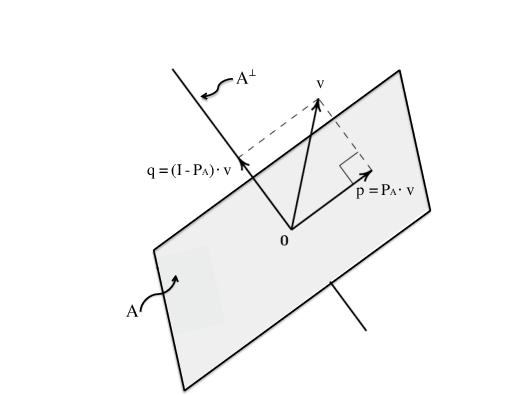
\includegraphics[width=10cm]{projection.png}
\caption{I took this figure off the internet so it's labelled differently but hopefully it's still understandable.}
\end{figure}

\textbf{Quick Problem.} Let $A$ be a matrix whose columns are the basis vectors of a vector space $V$ and $B$ be a matrix whose columns are the basis vectors of $V^{\perp}$. What does $A^TB$ look like?

%\textbf{Solution.} Say $V$ has $r$ basis vectors $v_i$ and $V^{\perp}$ has $n-r$ basis vectors $w_j$. Then each entry of $A^TB$ is $v_i \cdot w_j$ which must be $0$ as they are orthogonal. So $A^TB$ is the $r \times (n-r)$ zero matrix.

\clearpage

\section{$Ax = b$}

\subsection{Fundamental Subspaces}
Say $A$ is an $m \times n$ matrix with rank $r$. Then as a recap of our four fundamental subspaces,
\begin{center}
\begin{tabular}{c|c|c|c|c}
& Column Space & (Right) Nullspace & Row Space & Left Nullspace\\
\hline
Definition & $\{ Ax \mid \forall \, x \in \mathbb{R}^n\}$ & $\{ x \mid Ax = 0\,\, \forall x \in \mathbb{R}^n\}$ & $\{ A^Tx \mid \forall \, x \in \mathbb{R}^m\}$ & $\{ x \mid A^Tx = 0\,\, \forall x \in \mathbb{R}^m\}$\\
Notation & $C(A)$ & $N(A)$ & $C(A^T)$ & $N(A^T)$\\
Containing space & $\mathbb{R}^m$ & $\mathbb{R}^n$ & $\mathbb{R}^n$ & $\mathbb{R}^m$\\
Dimension & $r$ & $n-r$ & $r$ & $m-r$\\
Orthogonal subspace & $N(A^T)$ & $C(A^T)$ & $N(A)$ & $C(A)$
\end{tabular}
\end{center}

In addition, we have the following facts
\begin{itemize}
\item \textbf{$C(AB) \subseteq C(A)$}\\
Intuitively, the column space corresponds to what vectors come out from the left in a matrix-vector product.
\item \textbf{$N(B) \subseteq N(AB)$}\\
Intuitively, the null space corresponds to what vectors go into the right in a matrix-vector product.
\item \textbf{$N(A^TA) = N(A)$}\\
As a corollary, $C(A^TA) = C(A^T)$ and the rank of $A^TA$ is the same as $A$.
\end{itemize}

\subsection{Holistic View}
%\textit{Keywords: full column rank, full row rank, rank-deficient}
There are a lot of cases in terms of solving $Ax=b$ or doing least squares. You should understand the reasoning for them all. Below is another way of interpreting various cases using the four fundamental subspaces.

In the equation $Ax = b$, we have the vector $x \in \mathbb{R}^n$ and the vector $b \in \mathbb{R}^m$. Since we know $C(A) \perp N(A^T)$ and they're both in $\mathbb{R}^m$, we can break $b$ into $b = b_C + b_N$ where $b_C \in C(A)$ and $b_N \in N(A^T)$. Similarly, we can break $x$ into $x = x_C + x_N$ where $x_C \in C(A^T)$ and $x_N \in N(A)$. Then the equation
$$Ax = A(x_C + x_N) = Ax_C =  b_C = b - b_N$$
captures the behaviour for both $Ax=b$ and minimizing least squares $||Ax-b||^2$. Note that $b_C$ and $b_N$ are constants.

\begin{itemize}
\item $x_C \in C(A^T)$ is a particular solution. In practice, we don't need our particular solution to be in the row space as $x_C$ is.
\item $x_N \in N(A)$ is any vector in the nullspace and can be added to generate infinitely many solutions if $\dim(N(A)) > 0$. This is true both for $Ax = b$ and for minimizing least squares.
\item $b_C \in C(A)$ is equal to the $A\hat{x}$ that minimizes $||A\hat{x}-b||^2$. Note that it is a constant, so we can immediately see $A\hat{x}$ is unique.
\item $b_N \in N(A^T)$ is the error $b - A\hat{x}$. If $b_N \neq 0$, then there are no solutions to $Ax = b$ and we must do least squares. Otherwise, there is at least one solution.
\end{itemize}

\subsection{Orthogonal Bases}
%\textit{Keywords: orthogonal bases}
In many of the eigenvector problems, we've needed to convert a given initial vector into a linear combination of eigenvectors. For example, for ODEs, we know eigenvectors $x_1, x_2, x_3$ and want to find coefficients $c_1, c_2, c_3$ such that a given $x(0) = c_1 x_1 + c_2 x_2 + c_3 x_3$. This is equivalent to a linear system $$\begin{pmatrix} x_1 & x_2 & x_3\end{pmatrix}\begin{pmatrix}c_1\\c_2\\c_3\end{pmatrix} = x(0).$$
We know how to solve for the coefficients then, by performing elimination on the system. However, we've also seen that often, $x_1, x_2, x_3$ are known to be orthogonal. In this case, there is another way of determining a coefficient $c_1$ without even needing to know $x_2$ and $x_3$. Say we only know $x_1$ but we know $x_1^Tx_2 = x_1^Tx_3$ = 0. Then
\begin{align*}
\begin{pmatrix} x_1 & x_2 & x_3\end{pmatrix}\begin{pmatrix}c_1\\c_2\\c_3\end{pmatrix} &= x(0)\\
x_1^T\begin{pmatrix} x_1 & x_2 & x_3\end{pmatrix}\begin{pmatrix}c_1\\c_2\\c_3\end{pmatrix} &= x_1^Tx(0)\\
\begin{pmatrix}x_1^T x_1 & x_1^T x_2 & x_1^T x_3\end{pmatrix}\begin{pmatrix}c_1\\c_2\\c_3\end{pmatrix} &= x_1^T x(0)\\
\begin{pmatrix}x_1^T x_1 & 0 & 0\end{pmatrix}\begin{pmatrix}c_1\\c_2\\c_3\end{pmatrix} &= x_1^T x(0)\\
(x_1^T x_1)c_1 &= x_1^T x(0)\\
c_1 &= \frac{x_1^Tx(0)}{x_1^Tx_1}.
\end{align*}
This may be a slightly different manner in how you did it, though it should all be equivalent. The point here is that if you know a vector orthogonal to most of the columns, you can pick out certain entries of the solution vector without doing elimination. This can be done when your matrix has orthogonal columns, but it can also be done in other cases: PSET 10 problem 1 for example.
\clearpage

\section{Square Matrices}
We've seen a lot of different terms for various square matrices. Here's a quick refresher! All of these definitions already assume the matrix is square with size $n \times n$.

\subsection{Based on Structure}
%\textit{Keywords: diagonal, upper triangular, lower triangular}
\begin{itemize}
\item \textbf{Diagonal matrix}\\
A matrix $D$ where entries apart from the diagonal entries are zero. Invertible iff all the diagonal entries are non-zero, in which case $D^{-1}$ is a diagonal matrix whose entries the reciprocal of $D$'s entries. Its eigenvalues are exactly the diagonal entries and the determinant is the product.
\item \textbf{Upper triangular matrix}\\
A matrix $U$ where all entries below the diagonal are zero. Invertible iff all the diagonal entries are non-zero, and $Ux = b$ can be solved by back-substitution. Its eigenvalues are exactly the diagonal entries and the determinant is the product.
\item \textbf{Lower triangular matrix}\\
A matrix $L$ where all entries above the diagonal are zero. Invertible iff all the diagonal entries are non-zero, and $Lx = b$ can be solved by forward-substitution. Its eigenvalues are exactly the diagonal entries and the determinant is the product.
\end{itemize}

\subsection{Related to Eigenstuff}
%\textit{Keywords: symmetric, Hermitian, positive (semi-)definite, diagonalizable, defective, Markov}

\begin{itemize}
\item \textbf{Diagonalizable matrix}\\
A matrix $A$ with $n$ linearly independent eigenvectors. Can be written in the form $X\Lambda X^{-1}$, where the columns of $X$ are $A$'s eigenvectors and the diagonal entries of $\Lambda$ are its eigenvalues. In other words, $A$ is similar to a diagonal matrix.
\item \textbf{Markov matrix}\\
A matrix $M$ with non-negative entries such that each column's entries sums to $1$. A Markov matrix is not guaranteed to be diagonalizable, but certain things are known about its eigenvectors and eigenvalues. It is guaranteed that $1$ is a (non-repeated) eigenvalue which has a single eigenvector known as the steady state vector. This eigenvector has non-negative entries and is typically scaled so that the entries sum to $1$ (as it represents a vector of probabilities). It is also guaranteed that all other eigenvalues $\lambda$ have magnitude $|\lambda| \le 1$. For eigenvectors corresponding to these other eigenvalues, their entries are guaranteed to sum to $0$. As there may be multiple eigenvalues $\lambda$ which have $|\lambda| = 1$, long-term oscillating behaviour is possible for $M^nv$.
\item \textbf{Positive Markov matrix}\\
A Markov matrix $M$ whose entries are strictly positive (does not include zero) rather than just non-negative (which included zero entries). The main difference is that it is guaranteed that $\lambda = 1$ is the only eigenvalue with absolute value $1$. Thus, the long-term behaviour of $M^nv$ is guaranteed to converge to the steady state vector assuming that $v$ is a probability vector whose entries sum to $1$.
\item \textbf{Symmetric matrix}\\
A matrix $A$ such that $A^T = A$. Guaranteed to be diagonalizable, and the eigenvalues are guaranteed to be real. Also, the eigenvectors can be chosen to form an orthonormal basis so that $X^{-1} = X^T$ (note that $X$ must be real).
\item \textbf{Hermitian matrix}\\
The complex analogue of symmetric matrices. A matrix $A$ such that $A^H = A$. Guaranteed to be diagonalizable, and the eigenvalues are guaranteed to be real. Also, the eigenvectors can be chosen to form an orthonormal basis so that $X^{-1} = X^T$.
\item \textbf{Positive definite matrix}\\
A Hermitian matrix $A$ such that $x^HAx \ge 0$ for all vectors $x \in \mathbb{C}^n$ and equality only holds for $x = 0$. Its eigenvalues $\lambda$ are strictly positive ($\lambda > 0$). $A$ can be written as $B^HB$ for some full column rank matrix $B$.
\item \textbf{Positive semi-definite matrix}\\
A Hermitian matrix $A$ such that $x^HAx \ge 0$ for all vectors $x \in \mathbb{C}^n$. Its eigenvalues $\lambda$ are non-negative ($\lambda \ge 0$). $A$ can be written as $B^HB$ for some matrix $B$.
\item \textbf{Negative definite matrix}\\
A Hermitian matrix $A$ such that $x^HAx \le 0$ for all vectors $x \in \mathbb{C}^n$ and equality only holds for $x = 0$. Its eigenvalues $\lambda$ are strictly negative ($\lambda < 0$). $A$ can be written as $-B^HB$ for some full column rank matrix $B$.
\item \textbf{Negative semi-definite matrix}\\
A Hermitian matrix $A$ such that $x^HAx \le 0$ for all vectors $x \in \mathbb{C}^n$. Its eigenvalues $\lambda$ are non-positive ($\lambda \le 0$). $A$ can be written as $-B^HB$ for some matrix $B$.
\end{itemize}



\subsection{Other}
%\textit{Keywords: orthogonal, unitary, projection, invertible, singular}

\begin{itemize}
\item \textbf{Orthogonal matrix}\\
A real matrix $A$ such that $A^TA = I$. In other words, its transpose is its inverse, so $A^{-1} = A^T$ and $AA^T = I$. Another equivalent definition is that it's a square matrix with orthonormal columns (not just orthogonal, it's a poor name). It also has orthonormal rows. Multiplying a vector by $A$ preserves the length of the vector. That is, $||x|| = ||Ax||$.
\item \textbf{Unitary matrix}\\
The complex version of orthogonal matrix. We prefer using this term over orthogonal matrix. A complex matrix $A$ such that $A^HA = I$. Most of the facts are similar. The one difference is its determinant can be any complex number with magnitude $1$, while the determinant of an orthogonal matrix must be $1$ or $-1$.
\item \textbf{Projection matrix}\\
A matrix $P$ which projects onto a given subspace $V$. The column space of $P$ is $V$ and the rank of $P$ is equal to $\dim(V)$. In particular, $P$ is invertible if and only if $P = I$ and $V = \mathbb{R}^n$. $P$ is also always symmetric and satisfies $P^2 = P$. It has a corresponding projection matrix, $I-P$, which projects onto $V^{\perp}$. If $A$ is an $n \times \dim(V)$ matrix whose columns are the basis vectors of $V$, then $P = A(A^TA)^{-1}A^T$. If we have an orthogonal basis $q_1, q_2, \ldots$, then $P = \frac{q_1q_1^T}{q_1^Tq_1} + \frac{q_2q_2^T}{q_2^Tq_2} + \ldots$.
\item \textbf{Invertible matrix}\\
A matrix $A$ with an inverse $A^{-1}$ such that $A^{-1}A = I$. As mentioned before, we also have $AA^{-1} = I$. $A$ is invertible if it has a non-zero determinant. Equivalently, $A$ must be full rank.
\item \textbf{Singular matrix}\\
A matrix $A$ which is not invertible.
\end{itemize}

\clearpage

\section{Defective Matrices}

An $n \times n$ matrix $A$ is defective if and only if any of the following equivalent conditions hold

\begin{itemize}
\item $A$ is not diagonalizable
\item There do not exist $n$ linearly independent eigenvectors of $A$
\item For some eigenvalue $\lambda$ of $A$, the algebraic multiplicity of $\lambda$ (order of root in the characteristic polynomial) is greater than the geometric multiplicity (dimension of the nullspace $N(A - \lambda I)$)
\item $A$ is similar to a matrix in Jordan form
\end{itemize}

The last condition implies that if $A$ is defective, it must not have $n$ distinct eigenvalues. The reverse is NOT true. It is possible for a matrix to have repeated roots yet still be diagonalizable -- the identity matrix is an example. It is also impossible for a defective matrix to be Hermitian or unitary (which includes real matrices which are symmetric or orthogonal). This fact is based on the spectral theorem which is beyond this course.

\subsection{Examples}
The simplest example of a defective matrix is $\begin{pmatrix}0 & 1\\0&0\end{pmatrix}$, though there are many others. If you're asked to write a defective matrix with a certain eigenvalue $\lambda$, you can start by writing a Jordan block with $\lambda$. That is, $$J = \begin{pmatrix}\lambda & 1 & & & \ldots\\& \lambda & 1 & \ldots &\\ \vdots & & &\\ & & & \lambda & 1 \\ & & & & \lambda \end{pmatrix}$$ is a defective matrix. If you don't want zero entries, remember that similar matrices preserve diagonalizable/defective-ness. So pick some invertible matrix $P$ and give $PJP^{-1}$.

\subsection{Matrix Powers}
%\textit{Keywords: asymptotic behaviour}

Say $\lambda$ is the largest eigenvalue of $A$ by magnitude. Typically, $A^n v$ follows $\lambda^n$ times some constant vector asymptotically. However, if $\lambda$'s algebraic multiplicity is greater than its geometric multiplicity, then the asymptotic behaviour of $A^nv$ changes. In particular, an $n \lambda^n$ is introduced. Most of the time, the extra $n$ term doesn't change the overall behaviour. For example, $n 0.999^n$ as $n\to \infty$ still goes to $0$. The one case where it does make a difference is when $|\lambda| = 1$. Then unlike $\lambda^n$, which either oscillates around the complex unit circle or stays at $1$, $n \lambda^n$ diverges to $\infty$, albeit slowly. So this is something to be aware of.

Similarly, say $e^{At}$ will depend on the eigenvalue $\lambda$ of $A$ with largest real part. If $\lambda$'s algebraic multiplicity is greater than its geometric multiplicity, then the asymptotic behaviour of $e^{At}v$ changes to $t e^{\lambda t}$. This changes the asymptotic behaviour when the real part of $\lambda$ is $0$ in a similar manner as the above.

\end{document}
